\documentclass[12pt,halfline,a4paper]{ouparticle}

\usepackage{booktabs}
\usepackage{xcolor}
\usepackage{graphicx}
\usepackage{caption}
\usepackage{subcaption}

\begin{document}

\title{Does the Gender Employment Gap Expand Due to Natural Disasters? Evidence from the Great East Japan Earthquake\break {}}

\author{%
\name{Tomoto Masuda}
\address{}}

\abstract{This study analyzes the impact of the Great East Japan Earthquake of March 2011 on the gender employment gap in Fukushima Prefecture. Employing an event study approach alongside a difference-in-differences (DID) methodology with fixed effects regression, this study examines the earthquake's influence on gender-based employment dynamics. Drawing on extensive prefectural economic statistical data and individual socio-economic attributes from sources such as the Japan General Social Survey (JGSS), the Open Survey Data Japan Household Panel Survey on Consumer Preferences and Satisfaction (JHPS-CPS), the National Census, and the Housing and Land Survey, this study assesses the long-term effects of the earthquake on the gender employment gap. {\color{red}The results indicate that, in contrast to the immediate aftermath, the long-term impacts on the gender employment gap have attenuated significantly. This convergence can be primarily attributed to two factors: persistent governmental initiatives aimed at promoting female labor force participation, and the economically rational adaptations of households in response to disruptions in community structures.}}

\date{\today}

\keywords{word1; word2; word3; and word4}

\maketitle

\tableofcontents

\section{Introduction}
\label{sec1}

How does a natural disaster impact gender disparities within the labor markets of the affected regions? Previous studies present mixed findings on the impact of natural disasters on gender inequality, with some research indicating that such disasters widen gender gaps while other studies suggest a narrowing of these gaps. The Great East Japan Earthquake of March 2011 presented a unique opportunity to examine the dynamics of labor market responses to significant external shocks. This study focuses on Fukushima Prefecture, an area profoundly affected by both the earthquake and subsequent nuclear incident, to analyze the short-term and long-term impacts on the gender employment gap.


To frame the analysis, this study employs a comprehensive theoretical household model that encompasses four key elements. First, this study considers household decision-making processes, where utility maximization drives choices about labor supply and participation. This model recognizes that households make complex decisions balancing immediate needs with long-term economic rationality, often leading to gendered patterns of labor market engagement.

Secondly, the model incorporates the concept of economic shocks and adaptation mechanisms. The immediate aftermath of the disaster likely triggered rapid changes in employment patterns. However, over time, households develop adaptation strategies, including adjustments in labor supply preferences, acquisition of new skills, and reallocation of household labor responsibilities.

Thirdly, this study acknowledges the crucial role of government policies in shaping labor market outcomes. The theoretical framework examines how interventions aimed at promoting gender equality in employment can mitigate the adverse effects of economic shocks. This study assesses the effectiveness of these policies in both the short and long term, recognizing that policy impacts may evolve over time.

Lastly, the model considers the impact of community structure on household decision-making. The earthquake and its aftermath significantly disrupted local infrastructure and social networks, potentially altering the context in which households make employment decisions. We posit that long-term community rebuilding efforts can influence labor market dynamics and potentially reshape gender roles within households and the broader community.

By integrating these four elements - household decision-making, economic shocks and adaptation, policy interventions, and community structure - our theoretical model provides a comprehensive framework for understanding the complex interplay of factors affecting the gender employment gap in the wake of a major disaster. This study aims to contribute to the broader literature on labor market resilience and gender dynamics in employment, offering insights that may be applicable to other contexts of significant economic disruption.



ジェンダー固有の影響とその経済的なメカニズムについて詳細に論じる。



This paper explores the mechanisms through which the Great East Japan Earthquake impacted gender employment gaps for men and women as follows: First, in the short-term immediately after the disaster, women's employment decreased more than men's, widening the gender gap. This can be attributed to the higher prevalence of non-regular employment among women compared to men, as well as women's role as risk buffers for household adjustments. However, in the longer run, women's employment recovered rapidly, narrowing the gender gap. This reversal can be explained by two factors: a delayed onset of government policies promoting women's employment opportunities, and previously non-employed women (engaged in domestic labor or assisting family businesses) entering the labor force to supplement household income in the aftermath of the earthquake.


“The ‘Act on Promotion of Women’s Participation and Advancement in the Workplace’ enacted in April 2016 has led to the development of an environment conducive to working women of child-rearing generations, with initiatives such as the introduction of a reduced working hours system, restrictions on overtime work, and the establishment of childcare facilities within companies.”


2016年4月に施行された「女性活躍推進法」により、短時間勤務制度や所定外労働の制限、託児所の社内設置など、子育て世代の女性が働きやすい環境づくりが進められた。

This paper presents theoretical household model to explain...







\begin{figure}
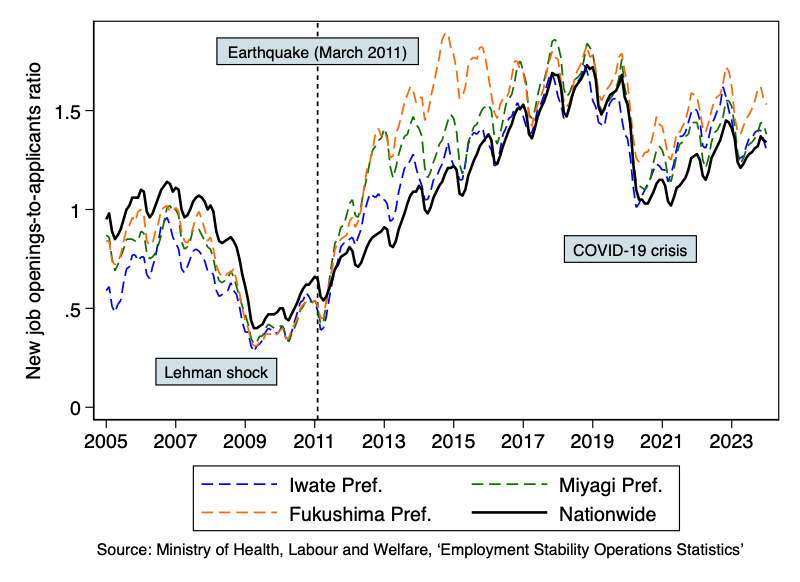
\includegraphics[width=\textwidth]{New job openings-to-applicants ratio.png}
\caption{New job openings-to-applicants ratio} \label{New job openings-to-applicants ratio.png}
\end{figure}


Public employment security office 

\begin{figure}
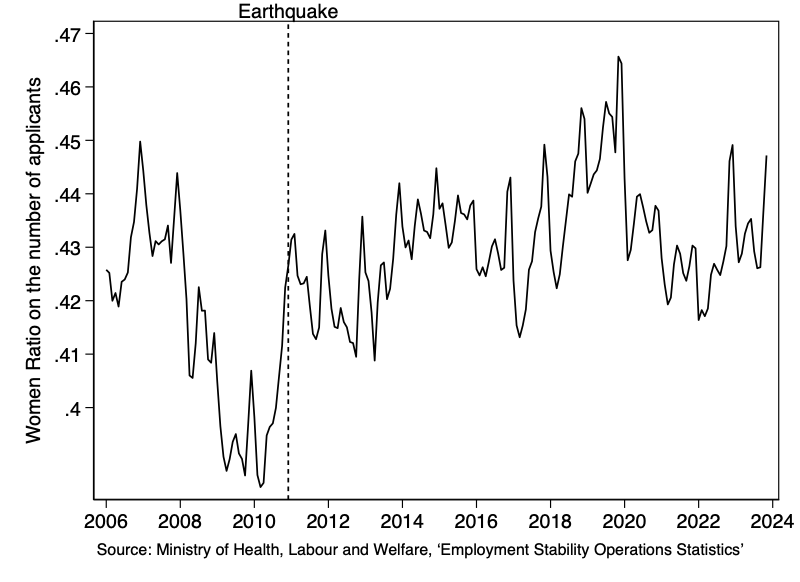
\includegraphics[width=\textwidth]{Women ratio on the number of applicants in Fukushima.png}
\caption{Women ratio on the number of applicants in Fukushima Pref.} \label{Women ratio on the number of applicants in Fukushima.png}
\end{figure}



\begin{figure}
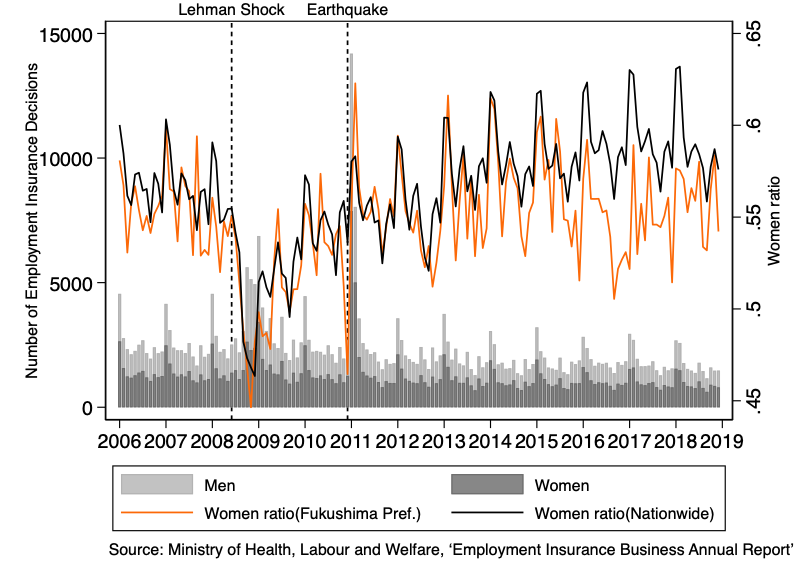
\includegraphics[width=\textwidth]{Number of Employment Insurance Decisions.png}
\caption{Number of Employment Insurance Decisions by gender in Fukushima Pref.} \label{Number of Employment Insurance Decisions.png}
\end{figure}


\begin{figure}
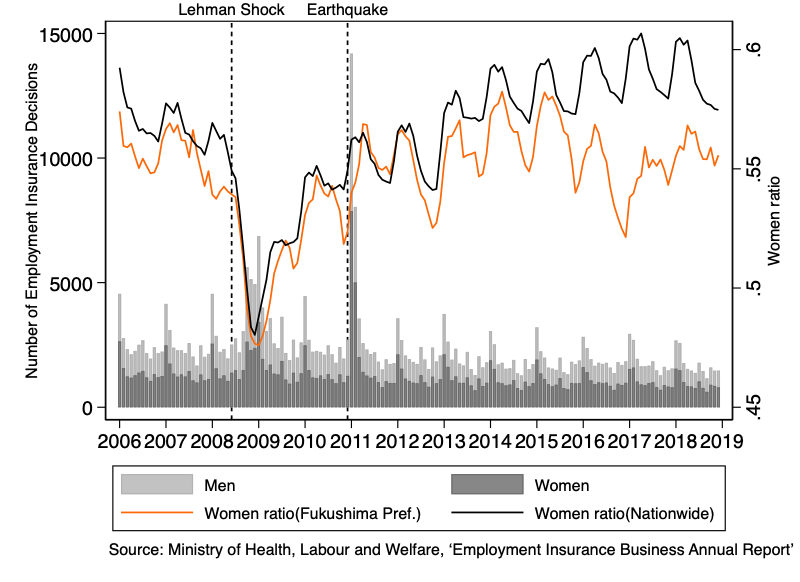
\includegraphics[width=\textwidth]{Number of Employment Insurance Decisions_2.png}
\caption{Number of Employment Insurance Decisions by gender in Fukushima Pref.} \label{Number of Employment Insurance Decisions_2.png}
\end{figure}



{
\def\sym#1{\ifmmode^{#1}\else\(^{#1}\)\fi}
\begin{tabular}{l*{1}{c}}
\hline\hline
            &\multicolumn{1}{c}{(1)}\\
            &\multicolumn{1}{c}{sbp}\\
\hline
age         &       0.739\sym{***}\\
            &     (0.034)         \\
[1em]
0.sex       &       0.000         \\
            &         (.)         \\
[1em]
1.sex       &       5.655\sym{***}\\
            &     (1.242)         \\
[1em]
1.race      &       0.000         \\
            &         (.)         \\
[1em]
2.race      &      -3.284         \\
            &     (4.748)         \\
[1em]
3.race      &      -6.955\sym{***}\\
            &     (2.560)         \\
[1em]
0.gender\_sex&       0.000         \\
            &         (.)         \\
[1em]
1.gender\_sex&      -0.685         \\
            &     (3.801)         \\
[1em]
2.gender\_sex&      -6.128         \\
            &     (6.345)         \\
[1em]
3.gender\_sex&       0.000         \\
            &         (.)         \\
[1em]
\_cons      &      98.283\sym{***}\\
            &     (2.720)         \\
\hline
\(N\)       &        1264         \\
\(R^{2}\)   &       0.282         \\
\hline\hline
\multicolumn{2}{l}{\footnotesize Standard errors in parentheses}\\
\multicolumn{2}{l}{\footnotesize \sym{*} \(p<0.1\), \sym{**} \(p<0.05\), \sym{***} \(p<0.01\)}\\
\end{tabular}
}


\section{Background}
\label{sec2}

\subsection{The Great East Japan Earthquake }
\label{sec5.1}

The Great East Japan Earthquake of March 2011 resulted in a tripartite catastrophe, comprising a magnitude 9.0 earthquake, a devastating tsunami, and a nuclear accident at the Fukushima Dai-ichi Nuclear Power plant. This disaster precipitated a severe humanitarian crisis, causing extensive damage particularly in the Iwate, Miyagi, and Fukushima prefectures in northeast Japan. According to the National Police Agency, 15,900 people lost their lives and 2,523 people remain unaccounted for, primarily as a result of the
massive tsunami that struck the eastern coast of Japan. The affected
prefectures account for 99.6\% of total fatalities and 99.8\% of total missing persons. In addition, a total of 3,784 fatalities and casualties were recognized as disaster-related deaths in Japan due to the exacerbation of chronic illnesses or suicide during evacuation. Approximately 90\% of fatalities were attributed to drowning. Table 1 presents a summary of the damages in the affected prefectures. The map below indicates the epicenter of the earthquake.

\begin{flushleft}
\begin{table}[h!]
  \caption{Direct Impact Overview in the Disaster-Stricken Prefectures}\label{table:disaster_situation}
  \begin{minipage}[c]{0.4\textwidth}
    \includegraphics[width=\textwidth,height=1.10\textwidth]{epicenter.jpeg}
  \end{minipage}
  \begin{minipage}[c]{0.48\textwidth}
    \raggedright
    \scalebox{0.8}{
    \begin{tabular}{|c|c|c|c|}
    \hline
    & \multicolumn{1}{c|}{Iwate} & \multicolumn{1}{c|}{Miyagi} & \multicolumn{1}{c|}{Fukushima} \\
    \hline
    Population & 1,330,147 & 2,348,165 & 2,029,064 \\
    Deceased & 4,675 & 9,544 & 1,614 \\
    Missing & 1,110 & 1,213 & 196 \\
    Fully destroyed houses & 20,185 & 83,932 & 20,136 \\
    Partially destroyed houses & 4,562 & 138,721 & 65,093 \\
    \hline
    \end{tabular}
    }
  \end{minipage}
\end{table}
\end{flushleft}

Fukushima Prefecture experienced a compound disaster involving both the tsunami triggered by the earthquake and the subsequent nuclear accident. The nuclear incident, in particular, necessitated large-scale evacuations, significantly disrupting local communities and labor markets. This unprecedented situation provides a unique context for examining the long-term socioeconomic impacts of compound disasters.




\subsection{Gender Gap in Japan}
\label{sec5.1}


According to the latest 2024 Global Gender Gap Report by the World Economic Forum (WEF), Japan ranks 118th out of 146 countries, placing it at the bottom among the G7 nations. Particularly, its rankings in the "Economic" and "Political" domains are notably low, with the "Economic" ranking being 120th out of 146 countries. Japan continues to exhibit substantial gender disparities in the economic sector, with the elimination of wage gaps remaining a significant challenge.


\section{DATA}
\label{sec5}

\subsection{DATA}
\label{sec5.1}

The main data used in the paper is Open Survey Data Japan Household Panel Survey on Consumer Preferences and Satisfaction (JHPS-CPS) collected by Osaka University under the 21st Century COE Program.


\section{Literature review}
\label{sec3}



Development economics models suggest an increase in household members’ labour supply as a shock-coping strategy which is associated with the narrowing of gender employment gaps. Several studies have documented a rise in female labor force participation following natural disasters. For instance, Canessa and Giannelli (2021) examine the impact of severe flooding in Bangladesh on women's employment and empowerment using georeferenced and longitudinal household panel data. Their difference-in-differences analysis reveals a significant 13 percentage point increase in women's employment probability post-flood. 


On the other hand, in labor economics, the Risk Adjustment Hypothesis posits that during economic shocks or natural disasters, women are more susceptible to labor market exclusion and face higher risks of deteriorating work conditions or unemployment compared to men. This hypothesis suggests that specific labor market subgroups, particularly female and non-regular workers, often function as 'adjustment valves,' absorbing economic shocks. These groups are disproportionately affected, serving as mechanisms to mitigate broader economic impacts. This framework illuminates the gender-based disparities in employment stability and the uneven distribution of economic resilience across worker categories during crises. For instance, Kim, Ashley, and Corcoran (2014) examines the economic impact of the 2010 earthquake in Haiti, focusing on changes in household composition and employment retention. Authors found that the earthquake caused a significant reduction in employment rates, from 52.6\% prior to the earthquake to 28.6\% five months post-event. Gender disparities were evident, with only 34.2\% of women retaining their employment compared to 55.6\% of men. 


The study tries to fill gaps in the still sparse literature on the impact of natural disasters on gender disparities by differentiating between short-term and long-term effects, addressing the contradictory findings of existing research that suggests either an exacerbation or a reduction of gender gaps.






\subsection{Document structure}
\label{sec3.3}

The main structure of your paper is as follows:

\begin{verbatim}
\documentclass[12pt,...]{ouparticle}
\usepackage[...]{packages}

\title{...}
\author{
    \name{...}
    \address{...}
    \email{...}
        \and
    \name{...}
    \address{...}
    \email{...}
        \and
    \name{...}
    \address{...}
    \email{...}
}
\abstract{...}
\keywords{...}

\maketitle

\begin{document}

\section{....}
...
\subsection{....}
....
\end{document}
\end{verbatim}


\subsection{Options}
\label{sec3.4}

By default, all of the options within \verb+article.cls+ are available
with this class file. This class file provides the following additional options.

\begin{description}
\item \textbf{oneline:}
This option will set your entire manuscript in one line spacing.
It will not affect the footnote, figure and table environments.

\item \textbf{halfline:}
This is to set your entire manuscript in half line spacing.

\item \textbf{endnotes:}
To make all footnotes to endnotes. You may follow the same
coding \verb+\footnote{text}+ for both footnotes and endnotes. Once you use this option
you have to use the \verb+\theendnotes+ command at the place where all the endnotes
have to be set in your paper.

\item \textbf{numbib:}
This is the default option that numbers the bibliography items;
this option does nothing with natbib and other packages.

\item \textbf{nonumbib:} For unnumbered bibliography.
\end{description}


\subsection{Front matter}
\label{sec3.5}

The title of the manuscript is simply specified by using the \verb+\title{text}+ command in
the same manner as in this sample. Author's information consists of the name of the author
and the corresponding institutions with addresses, as given in this example. Include an
electronic mail address if available, inserting it into the \verb+\email{text}+ commands.
You may follow the same coding if there are more than one author; separate authors with
\verb+\and+. Please identify the corresponding author with his/her electronic
mail address by \verb+\thanks{text}+. An abstract for your paper is specified by using
\verb+\abstract{text}+. A \verb+\keywords{text}+ macro may also be used to indicate keywords for the
article. Use \verb+\maketitle+ after the abstract and keywords to make the header of your article.

\subsection{Sections and subsections}
\label{sec3.6}

To begin a new section, give the heading of that section in the \verb+\section{text}+ command.
A section number is supplied automatically. Use the starred form (\verb+\section*{text}+) of the
command to suppress the automatic numbering. If you want to be able to make reference to that section,
then you need to \texttt{label} it (see Section \ref{sec3.14}). You can have sections up to
five levels. The sectioning commands are \verb|\section|, \verb|\subsection|, \verb|\subsubsection|,
\verb|\paragraph| and \verb|\subparagraph|.

\subsection{Ordinary text}
\label{sec3.7}

The ends of words and sentences are marked by spaces. It does not matter how many
spaces you type. The end of a line counts as a space. One
or more blank lines denote the end of a paragraph.

There are a number of things for which you need to follow different
methods. As you know, quotation marks, quotes within quotes,
dashes, ellipsis, etc. should be as per the \LaTeX\ standard input. \LaTeX\ interprets some
common characters as commands, and therefore you must instead type those common characters as
specific \LaTeX\ commands to generate them. Those characters are \$, \&, \%, \#, \{, and \}.

\subsection{Formatting}
\label{sec3.8}

One should always use \LaTeX\ macros rather than the lower-level
\TeX\ macros like \verb+\it+, \verb+\bf+ and \verb+\tt+. The
\LaTeX\ macros offer much improved features. The following table summarizes the font
selection commands in \LaTeX.


\subsubsection*{\LaTeX\ text formatting commands}
\begin{tabular}{ll@{\hskip60pt}ll}
\verb+\textit+  & Italics      &\verb+\textsf+  & Sans Serif\\
\verb+\textbf+  & Boldface     &\verb+\textsc+  & Small Caps\\
\verb+\texttt+  & Typewriter   &\verb+\textmd+  & Medium Series\\
\verb+\textrm+  & Roman        &\verb+\textnormal+ & Normal Series\\
\verb+\textsl+  & Slanted      &\verb+\textup+  & Upright Series
\end{tabular}


\subsubsection*{\LaTeX\ math formatting commands}
\begin{tabular}{ll@{\qquad}ll}
\verb+\mathit+     & Math Italics            &\verb+\mathfrak+   & Fraktur\\
\verb+\mathbf+     & Math Boldface       &\verb+\mathbb+     & Blackboard Bold\\
\verb+\mathtt+     & Math Typewriter     &\verb+\mathnormal+ & Math Normal\\
\verb+\mathsf+     & Math Sans Serif     &\verb+\boldsymbol+ & Bold math for Greek letters\\
\verb+\mathcal+    & Calligraphic        &                   & and other symbols
\end{tabular}


\subsection{Figures and tables}
\label{sec3.9}

Use normal \LaTeX\ coding for figures and tables.
Figure and table environments should be inserted after (not in) the paragraph in which
the figure is first mentioned or grouped all
together at the end of the file. They will be numbered automatically.
The following is an example of typesetting a table.

\begin{verbatim}
\begin{table}
\caption{Table caption text.}
\label{key}
The table matter goes here.
\end{table}
\end{verbatim}

As always with \LaTeX, the \verb+\label+ must be after the
\verb+\caption+, and inside the figure or table environment. The reference for
figures and tables inside text can be made using the \verb|\ref{key}| command.


\subsection{Equations}\label{sec3.10}

Equations are used in the same way as described in the \LaTeX\ manual.
Do not start a paragraph with a displayed equation. Equations are numbered consecutively, with equation numbers
in parentheses flush right.
 For example, if you type
\begin{verbatim}
\begin{equation}\label{eq1}
\int^{r_2}_0 F(r,\varphi){\rm d}r\,{\rm d}\varphi = [\sigma r_2/(2\mu_0)]
\int^{\infty}_0\exp(-\lambda|z_j-z_i|)\lambda^{-1}J_1 (\lambda r_2)J_0
(\lambda r_i\,\lambda {\rm d}\lambda)
\end{equation}
\end{verbatim}
then you will get the following output:
\begin{equation}\label{eq1}
\int^{r_2}_0 F(r,\varphi){\rm d}r\,{\rm d}\varphi = [\sigma r_2/(2\mu_0)]\int^{\infty}_0
\exp(-\lambda|z_j-z_i|)\lambda^{-1}J_1 (\lambda r_2)J_0 (\lambda r_i\,\lambda {\rm d}\lambda)
\end{equation}
It inserts space both above and below the equation. \AmS-\LaTeX{} has several environments that
make it easier to typeset complicated multiline displayed equations. These are explained in the
\AmS-\LaTeX{} User Guide. A \verb+subequation+ environment is available to create equations with
sub-numbering of the equation counter. It takes one (optional)
argument to specify the way that the sub-counter should appear.


\subsection{Displayed text}
\label{sec3.11}

Text is displayed by indenting it from the left and right margins.
Quotations are commonly displayed. There are short
quotations:
\begin{quote}
   This is a short quotation.  It consists of a
   single paragraph of text.  See how it is formatted.
\end{quote}
and longer ones:
\begin{quotation}
   This is a longer quotation.  It consists of two
   paragraphs of text, neither of which are
   particularly interesting.

   This is the second paragraph of the quotation.  It
   is just as dull as the first paragraph.
\end{quotation}
You can even display poetry.
\begin{verse}
   There is an environment
    for verse \\             % The \\ command separates lines
   Whose features some poets % within a stanza.
   will curse.

                             % One or more blank lines separate stanzas.

   For instead of making\\
   Them do \emph{all} line breaking, \\
   It allows them to put too many words on a line when they'd rather be
   forced to be terse.
\end{verse}


\subsection{Listings}
\label{sec3.12}

Another frequently displayed structure is a list. The
following is an example of an \emph{itemized} list.
\begin{itemize}
   \item This is the first item of an itemized list.
         Each item in the list is marked with a
         `$\bullet$'.

   \item This is the second item of the list. It
         contains another list nested inside it. The
         inner list is an \emph{enumerated} list.
         \begin{enumerate}
            \item This is the first item of an enumerated
                  list that is nested within the
                  itemized list.

            \item This is the second item of the inner list.
                  \LaTeX\ allows you to nest lists
                  deeper than you really should.
         \end{enumerate}
         This is the rest of the second item of the
         outer list. It is no more interesting than
         any other part of the item.
   \item This is the third item of the list.
\end{itemize}


\subsection{Displayed sentences: theorems and such}
\label{sec3.13}

These environments have to be defined with the help of \LaTeX's \verb+\newtheorem+ command, and
also with the \AmS-\LaTeX\ package for theorems that is already with your class file.
For example, \verb+\newtheorem{thm}{Theorem}+. Predefined theorem styles can be used in your article
to differentiate the theorem-like environments. You can have an extra command, \verb+\newproof+,
that can be used for displayed text. The following is an example of using the above-defined
\verb+thm+ environment.
\begin{verbatim}
\begin{thm}
This is body matter for this environment.
\end{thm}
\end{verbatim}

\subsection{Cross-referencing}
\label{sec3.14}

\LaTeX\ possesses features for labelling and cross-referencing
section headings, equations, tables, figures and theorems.
Their proper usage in the context of section headings, equations,
tables and figures are discussed in the appropriate sections.

Cross-referencing depends upon the use of `keys' that are defined by the user.
The \verb+\label{key}+ command is used to identify the links. Keys are strings of
characters that serve to label section headings, equations, tables and figures
that replace explicit, by-hand numbering. The \verb+\ref{key}+ command is used for
cross-referencing.

Files that use cross-referencing (and almost all manuscripts do)
need to be processed through \LaTeX\ at least twice to
ensure that the keys have been properly linked to the appropriate numbers.

\subsection{Footnotes and endnotes}
\label{sec3.15}

The footnote text can either appear at the bottom of a page or at the end of your paper.
The \verb+\footnote+ macro \emph{should not} be used in the front matter to provide additional
information about authors (such as corresponding addresses); instead, use \verb+\thanks{text}+ commands.
The document option `\texttt{endnotes}' is used to make endnotes. The command \verb+\theendnotes+ should
be used to place the endnotes at the required location in the text. They will be put in a separate
`Notes' section.


\subsection{Appendix}
\label{sec3.16}

The \verb+\appendix+ command signals that all following sections are
appendices, and therefore the headings after \verb+\appendix+ will be set
as appendix headings. For a single appendix, use \verb+\appendix*+ followed by the \verb+\section{text}+
command to suppress the appendix letter in the section heading.


\subsection{Special sections for notes and acknowledgements}
\label{sec3.17}

If you wish to include a `Notes' or `Acknowledgements' section in your paper,
use the \verb+\begin{notes}...\end{notes}+ macro. We use the same environment for both
`Notes' and `Acknowledgements'. The following examples show to how to use this macro.
\begin{verbatim}
\begin{notes}
Please note that this class file is provided as it is, and
copyright by Oxford University Press. You are free to use this
class file, provided that you do not make changes in this class file.
If you do make changes, you are requested to rename the class file.
\end{notes}

\begin{notes}[Acknowledgements]
The authors would like to thank...
\end{notes}

\end{verbatim}



\section{Data and Descriptive Statistics}
\label{sec4}

This study utilizes the exogeneity of the impact of the Great East Japan Earthquake to conduct a regression analysis.




\begin{verbatim}
amsmath         graphicx
amssymb         endnotes
amsfonts        setspace
verbatim        geometry
\end{verbatim}

The commonly used packages already used by this class file that authors can use whenever required are:
\begin{verbatim}
xspace          latexsym        url
amscd           multicol        algorithm
rotating        array           subfigure
\end{verbatim}

Additionally, you can use other packages and these should be loaded
using the \verb+\usepackage+ command.




\section{Results}
\label{sec5}

\subsection{Results}
\label{sec5.1}


Initially, these events disproportionately impacted women workers negatively. However, The earthquake and nuclear disaster potentially accelerated women's labor market participation by fundamentally disrupting communities bound by traditional gender roles. In the short term, the disaster and nuclear accident had a more severe negative impact on female workers. However, in the long term, this catastrophic event, while devastating, may have inadvertently challenged long-standing societal norms, thus facilitating increased female workforce engagement.



\section{References}
\label{sec5}


The reference entries can be \LaTeX\ typed bibliographies or generated through a BIB\TeX\ database.
BIB\TeX\ is an adjunct to \LaTeX\ that aids in the preparation of bibliographies. BIB\TeX\
allows authors to build up a database or collection of bibliography entries that may be used for many
manuscripts. They also save us the trouble of having to specify formatting. More details can be found
in the \textit{BIB\TeX\ Guide}. For \LaTeX\ reference entries use the
\verb+\begin{thebibliography}....\end{thebibliography}+ environment (see below) to make references in your paper.
We have provided the class file option to distinguish two styles of references. Those options are \verb+numbib+ and \verb+nonumbib+.
You can select one of these options with the \verb+\documentclass+ command. By default the class file will take the
\verb+numbib+ option. The following is an example of \LaTeX\ bibliography.

\begin{verbatim}
\begin{thebibliography}{0}
\bibitem{bib1}
Goossens, M., F. Mittelbach, and A. Samarin: {\em The {\LaTeX} Companion}.
Addison-Wesley, Reading, MA, USA, 1994.
\bibitem{bib2}
Knuth, D.E: {\em The {\TeX}book}. Addison-Wesley, Reading, MA, USA, 1984.
\bibitem{bib3}
Lamport, L.: {\em {\LaTeX} -- A Document Preparation System -- User's
Guide and Reference Manual}. Addison-Wesley, Reading, MA, USA, 1985.
\bibitem{bib4}
Smith, I.N., R.S. Johnes, and W.P. Hines: 1992, `Title of the Article',
\textit{Journal Title in Italics} \textbf{Vol. no. X}, pp. 00--00
\end{thebibliography}
\end{verbatim}


\begin{table}[htbp]\centering
\def\sym#1{\ifmmode^{#1}\else\(^{#1}\)\fi}
\caption{Example 1}
\begin{tabular}{l*{4}{D{.}{.}{-1}}}
\toprule
            &\multicolumn{1}{c}{(1)}         &\multicolumn{1}{c}{(2)}         &\multicolumn{1}{c}{(3)}         &\multicolumn{1}{c}{(4)}         \\
            &        POLS         &     Between         &          FE         &          RE         \\
\midrule
$\mathit{grade}$&       0.063\sym{***}&       0.061\sym{***}&       0.000         &       0.065\sym{***}\\
            &     (0.001)         &     (0.002)         &         (.)         &     (0.002)         \\
\addlinespace
$\mathit{age}$&       0.039\sym{***}&       0.032\sym{***}&       0.036\sym{***}&       0.037\sym{***}\\
            &     (0.003)         &     (0.009)         &     (0.003)         &     (0.003)         \\
\addlinespace
$\mathit{age}^2$&      -0.001\sym{***}&      -0.001\sym{***}&      -0.001\sym{***}&      -0.001\sym{***}\\
            &     (0.000)         &     (0.000)         &     (0.000)         &     (0.000)         \\
\addlinespace
$\mathit{exp}$&       0.021\sym{***}&       0.014\sym{**} &       0.033\sym{***}&       0.029\sym{***}\\
            &     (0.002)         &     (0.006)         &     (0.003)         &     (0.002)         \\
\addlinespace
$\mathit{exp}^2$&       0.000\sym{***}&       0.001\sym{**} &       0.000\sym{*}  &       0.000\sym{***}\\
            &     (0.000)         &     (0.000)         &     (0.000)         &     (0.000)         \\
\addlinespace
$\mathit{tenure}$&       0.047\sym{***}&       0.070\sym{***}&       0.036\sym{***}&       0.039\sym{***}\\
            &     (0.002)         &     (0.006)         &     (0.002)         &     (0.002)         \\
\addlinespace
$\mathit{tenure}^2$&      -0.002\sym{***}&      -0.003\sym{***}&      -0.002\sym{***}&      -0.002\sym{***}\\
            &     (0.000)         &     (0.000)         &     (0.000)         &     (0.000)         \\
\addlinespace
$\alpha$    &       0.247\sym{***}&       0.334\sym{***}&       1.037\sym{***}&       0.239\sym{***}\\
            &     (0.049)         &     (0.121)         &     (0.049)         &     (0.049)         \\
\midrule
\(N\)       &       28091         &       28091         &       28091         &       28091         \\
\(R^{2}\)   &       0.375         &       0.490         &       0.173         &                     \\
\bottomrule
\multicolumn{5}{l}{\footnotesize Standard errors in parentheses}\\
\multicolumn{5}{l}{\footnotesize \sym{*} \(p<0.1\), \sym{**} \(p<0.05\), \sym{***} \(p<0.01\)}\\
\end{tabular}
\end{table}



\end{document}